\section{Methodology}\label{sec:methods}

\subsection{Framework Overview}\label{subsec:framework}

Our hybrid causal ML pipeline addresses three fundamental challenges in policy evaluation: (1) identifying true causal relationships from observational data, (2) estimating effects amid complex confounding, and (3) forecasting policy impacts under uncertainty. This section presents our end-to-end workflow.

\subsection{Methodological Overview}\label{subsec:methodology_overview}

Figure~\ref{fig:modelplan} provides a visual overview of the proposed hybrid causal machine learning framework, illustrating the integration of LSTM forecasting, DoubleML causal estimation, and Causal Forest heterogeneity modeling within the VAT policy evaluation pipeline.

\begin{figure}[htbp]
    \centering
    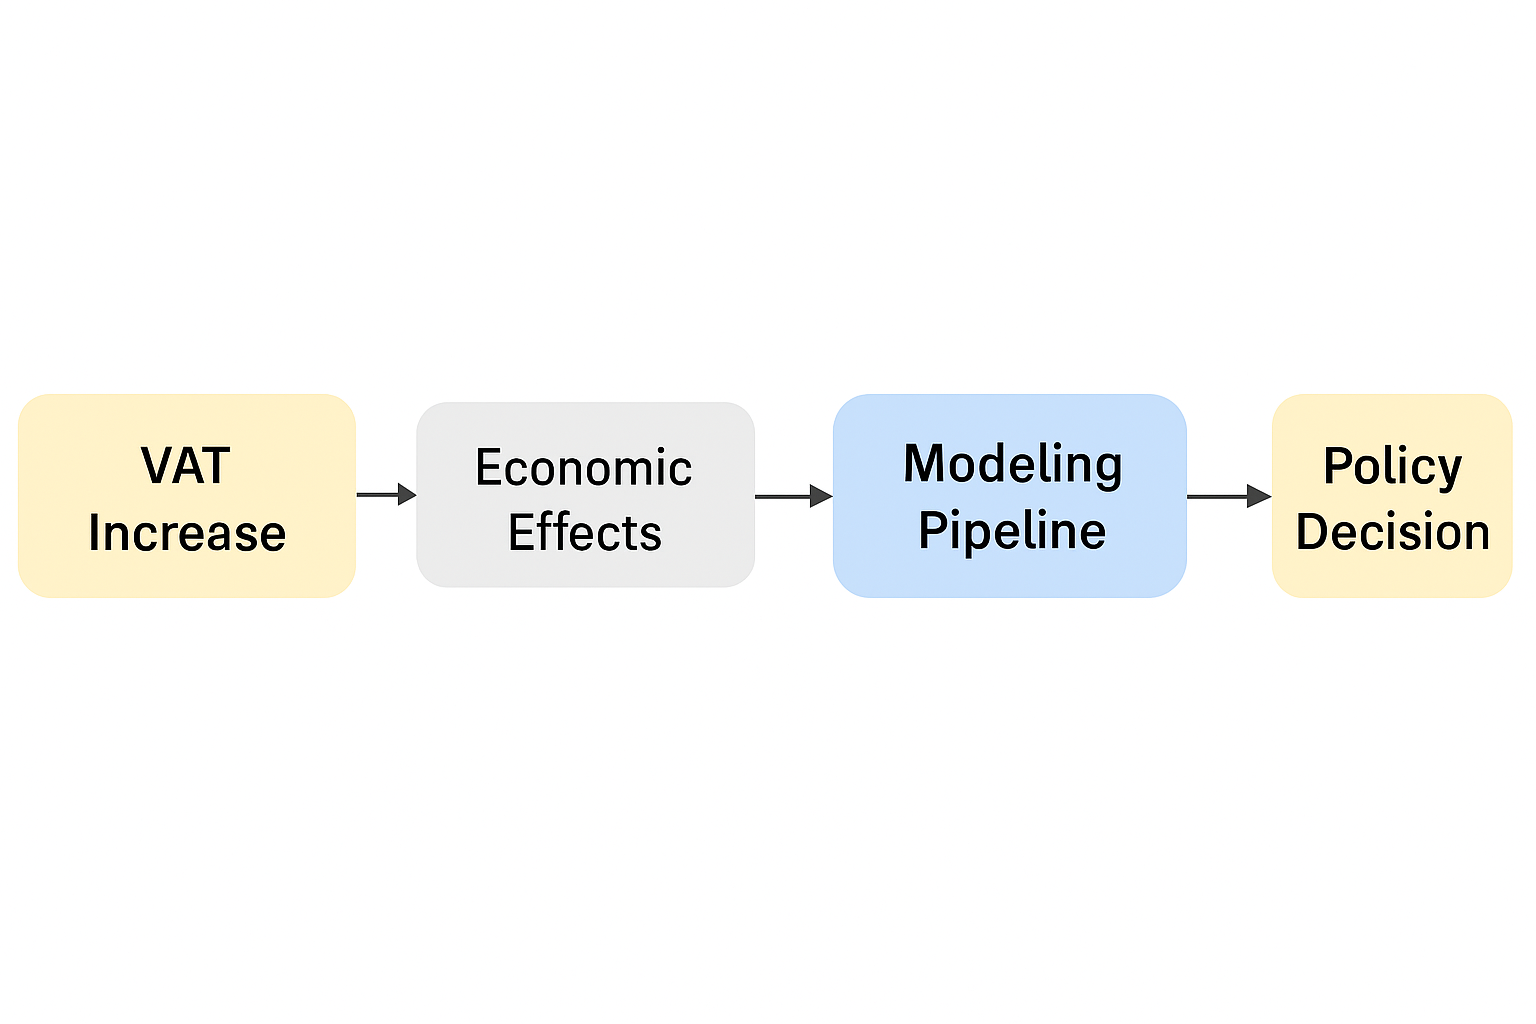
\includegraphics[width=\textwidth]{images/modelplan.png}
    \caption{Hybrid Causal Machine Learning Framework for VAT Policy Analysis}
    \label{fig:modelplan}
\end{figure}



\subsubsection{Stage 1: Causal Discovery}
\textbf{Rationale:} Traditional econometric models often assume known causal structures. We instead use data-driven discovery to uncover the actual relationships between VAT policy and economic outcomes.

\textbf{Implementation:}
\begin{itemize}
    \item \textbf{PC Algorithm}: This constraint-based approach iteratively examines pairs of variables and removes direct causal links when conditional independence is detected.
    \item \textbf{FCI Extension}: The Fast Causal Inference algorithm extends the basic PC approach by accounting for potential latent confounders.
    \item \textbf{Validation Strategy}: We employ bootstrap resampling with 100 iterations, retaining only causal relationships that appear consistently across at least 90\% of bootstrap samples.
\end{itemize}

\subsection{Double Machine Learning (DoubleML)}\label{subsec:doubleml}
\begin{figure}[H]
    \centering
    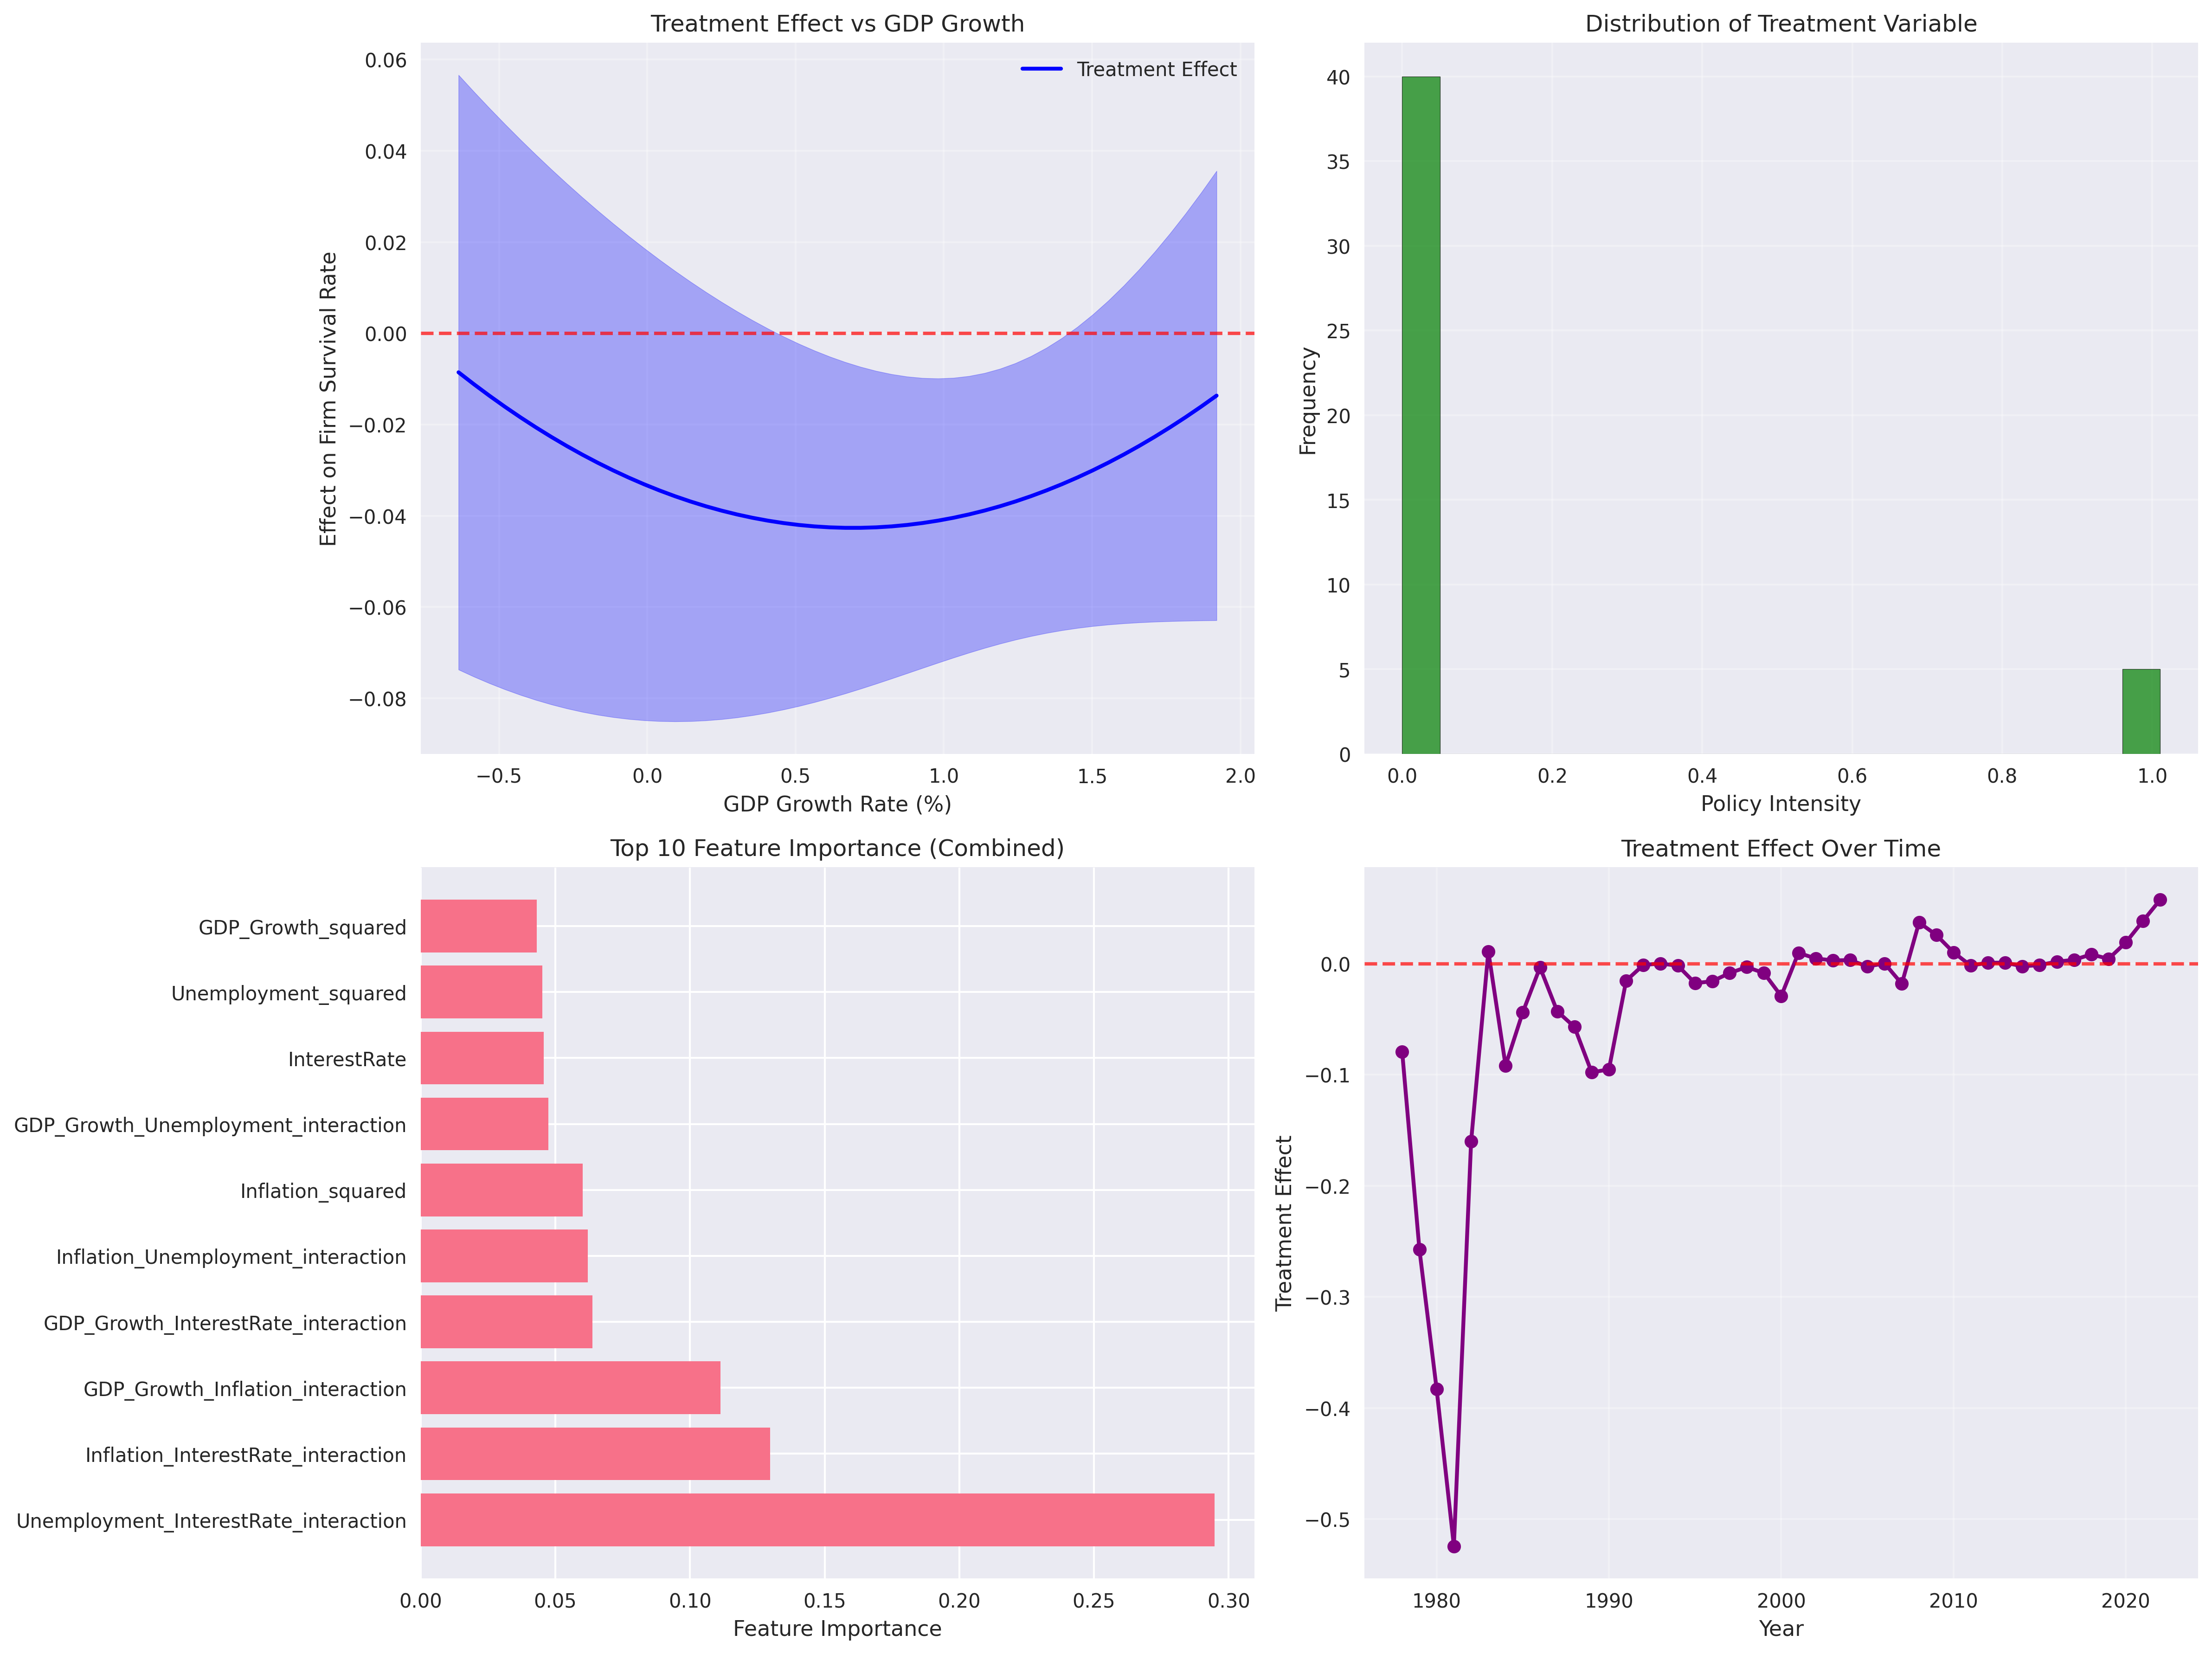
\includegraphics[width=\textwidth]{figures/dml_analysis_results.png}
    \caption{DoubleML Causal Effect Estimation Results}
    \label{fig:dml_analysis_results}
\end{figure}
\subsubsection{Core Principle}
The fundamental innovation of DoubleML lies in its orthogonalization approach, which separates the estimation of treatment effects from nuisance parameters. This prevents regularization bias that commonly affects traditional high-dimensional econometric models.

\subsubsection{Implementation Process}
\begin{enumerate}
    \item \textbf{Nuisance Function Estimation}: The outcome model captures how control variables predict outcomes in the absence of treatment. The propensity model estimates the likelihood of receiving treatment given observed characteristics.
    \item \textbf{Orthogonalization Process}: This step creates residualized versions of both outcomes and treatment assignments by removing the predictable components based on control variables.
    \item \textbf{Final Effect Estimation}: The causal effect is estimated using the orthogonalized variables, yielding unbiased treatment effect estimates with proper statistical inference.
\end{enumerate}


\subsection{LSTM Time-Series Model}\label{subsec:lstm}



\subsubsection{Theoretical Motivation}
\begin{figure}[H]
    \centering
    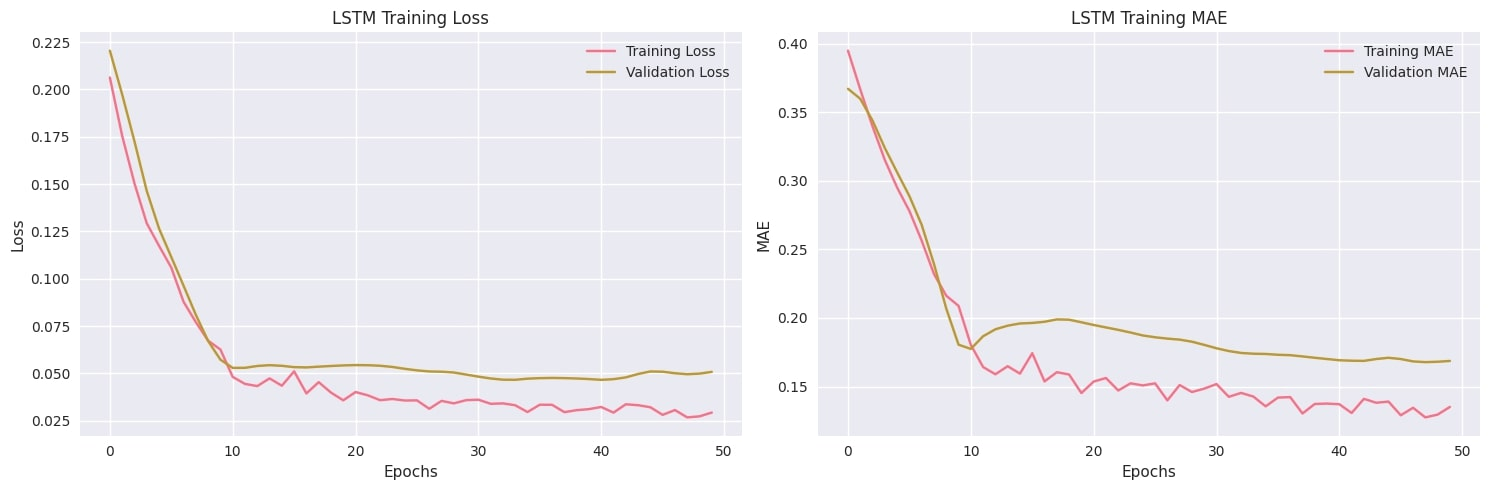
\includegraphics[width=0.9\textwidth]{figures/lstm.jpg}
    \caption{LSTM Network Economic Time-Series Forecasting result}
    \label{fig:lstm_architecture}
\end{figure}

Traditional time-series methods like ARIMA assume linear relationships and struggle with complex, multi-scale dependencies common in economic data. LSTM networks excel at capturing long-term dependencies while avoiding the vanishing gradient problem.

\subsubsection{Architecture Design}
The LSTM architecture incorporates three key gating mechanisms:
\begin{itemize}
    \item \textbf{Forget Gate}: Determines which information from previous time steps should be discarded
    \item \textbf{Input Gate}: Controls which new information should be stored in the cell state
    \item \textbf{Output Gate}: Regulates which parts of the cell state should influence the current output
\end{itemize}

\textbf{Mathematical Formulation:}
\begin{align}
  f_t &= \sigma(W_f [h_{t-1}, x_t] + b_f), \\
  i_t &= \sigma(W_i [h_{t-1}, x_t] + b_i), \\
  \tilde{c}_t &= \tanh(W_c [h_{t-1}, x_t] + b_c), \\
  c_t &= f_t \odot c_{t-1} + i_t \odot \tilde{c}_t, \\
  o_t &= \sigma(W_o [h_{t-1}, x_t] + b_o), \\
  h_t &= o_t \odot \tanh(c_t)
\end{align}

\subsubsection{Training Protocol}
The training protocol incorporates several advanced techniques:
\begin{itemize}
    \item \textbf{Teacher Forcing}: Randomly uses ground truth versus model predictions during training to improve generalization
    \item \textbf{Robust Loss Function}: Huber loss combines advantages of mean squared error and mean absolute error
    \item \textbf{Regularization Strategy}: Layer normalization and dropout prevent overfitting while maintaining model expressiveness
\end{itemize}

\subsection{Causal Forests}\label{subsec:cforests}

\subsubsection{Causal Forest Results}
The following figure presents the causal forest analysis results, illustrating the heterogeneous treatment effects across different subgroups and covariates:

\begin{figure}[H]
    \centering
    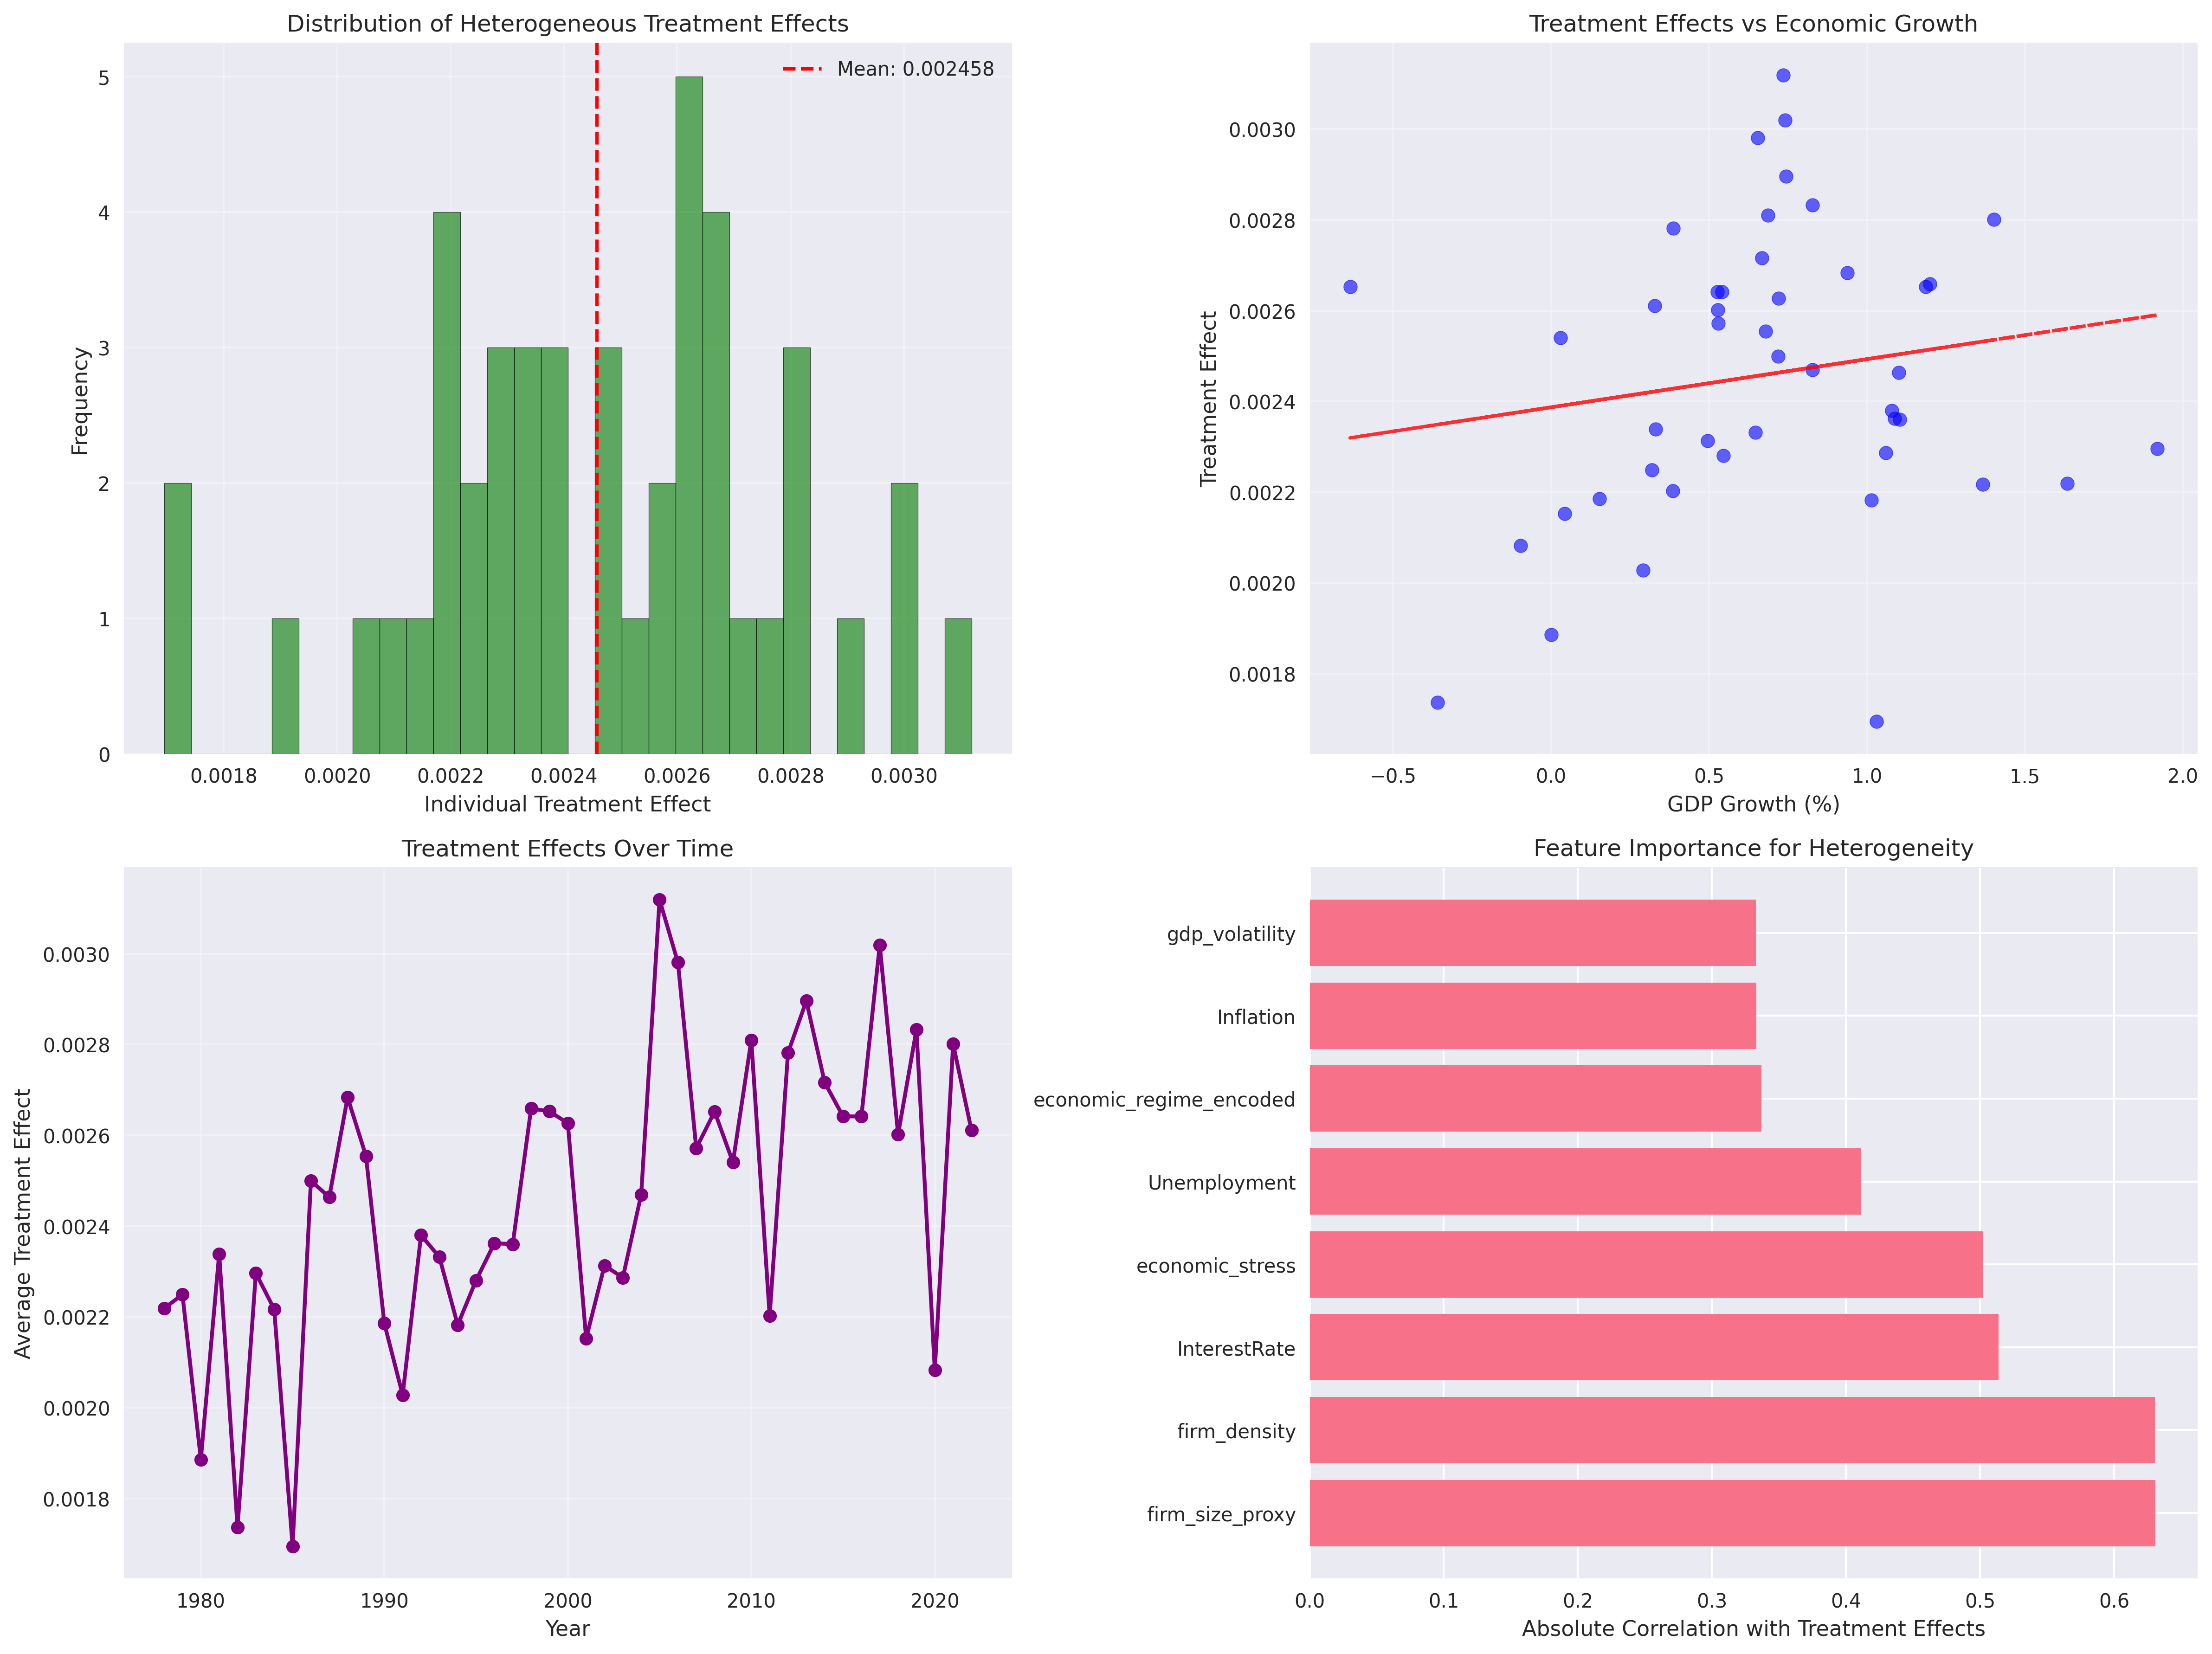
\includegraphics[width=\textwidth]{figures/causal_forest_results.png}
    \caption{Causal Forest Analysis Results}
    \label{fig:causal_forest_results}
\end{figure}


\subsubsection{Theoretical Foundation}
Causal Forests extend random forest methodology to identify treatment effect heterogeneity without requiring researchers to pre-specify relevant subgroups. This data-driven approach discovers how policy effects vary across different contexts automatically.

\subsubsection{Methodological Approach}
\textbf{Honest Splitting}: The algorithm uses different subsamples for determining split points and estimating treatment effects within each leaf, ensuring unbiased effect estimates.

\textbf{Effect Estimation}: The estimator aggregates tree-level localized differences:
\begin{equation}
  \hat{\tau}(x) = \sum_{b=1}^B w_b(x) \left( \bar{y}_{b,1} - \bar{y}_{b,0} \right)
\end{equation}
where $w_b(x)$ weights tree $b$ leaves containing $x$.

\subsection{Heterogeneous Treatment Effects Analysis}\label{subsec:heterogeneous}

\subsubsection{Treatment Definition}
VAT policy changes are treated as binary interventions, where firms and economic units are considered "treated" when experiencing VAT rate increases above a specified threshold.

\subsubsection{Estimation Approach}
The Causal Forest algorithm estimates conditional average treatment effects by:
\begin{itemize}
    \item Partitioning the covariate space based on treatment effect heterogeneity
    \item Using honest splitting to ensure unbiased effect estimates within each partition
    \item Averaging outcomes from similar units weighted by their proximity in the covariate space
\end{itemize}

\subsection{Ensemble Framework and Policy Optimization}\label{subsec:hybrid}

\subsubsection{Adaptive Weighting Strategy}
The ensemble dynamically adjusts component weights based on contextual factors:
\begin{itemize}
    \item \textbf{Temporal Relevance}: LSTM predictions receive higher weight for recent time periods
    \item \textbf{Heterogeneity Context}: Causal Forest estimates are emphasized when analyzing subgroups where treatment effects vary significantly
    \item \textbf{Confounding Complexity}: DoubleML receives priority in high-dimensional settings
\end{itemize}

\subsection{Benchmarking Against Traditional Methods}\label{subsec:benchmark}

\subsubsection{Comparative Framework Design}
We implement comprehensive comparisons against standard econometric methods including ordinary least squares (OLS) and difference-in-differences (DiD) specifications.

\subsubsection{Performance Evaluation Framework}
We assess model performance across multiple dimensions:
\begin{itemize}
    \item \textbf{Predictive Accuracy}: Out-of-sample prediction quality measured through mean squared error
    \item \textbf{Bias Reduction}: Comparison of estimated effects against known benchmarks
    \item \textbf{Confidence Interval Coverage}: Statistical reliability of uncertainty quantification
    \item \textbf{Policy Regret}: Expected loss from suboptimal policy choices based on model recommendations
\end{itemize}


\subsubsection{Complete Hybrid Model Architecture}
The following figure illustrates the complete integration of all methodological components within our hybrid causal machine learning framework:
\begin{figure}[htbp]
    \centering
    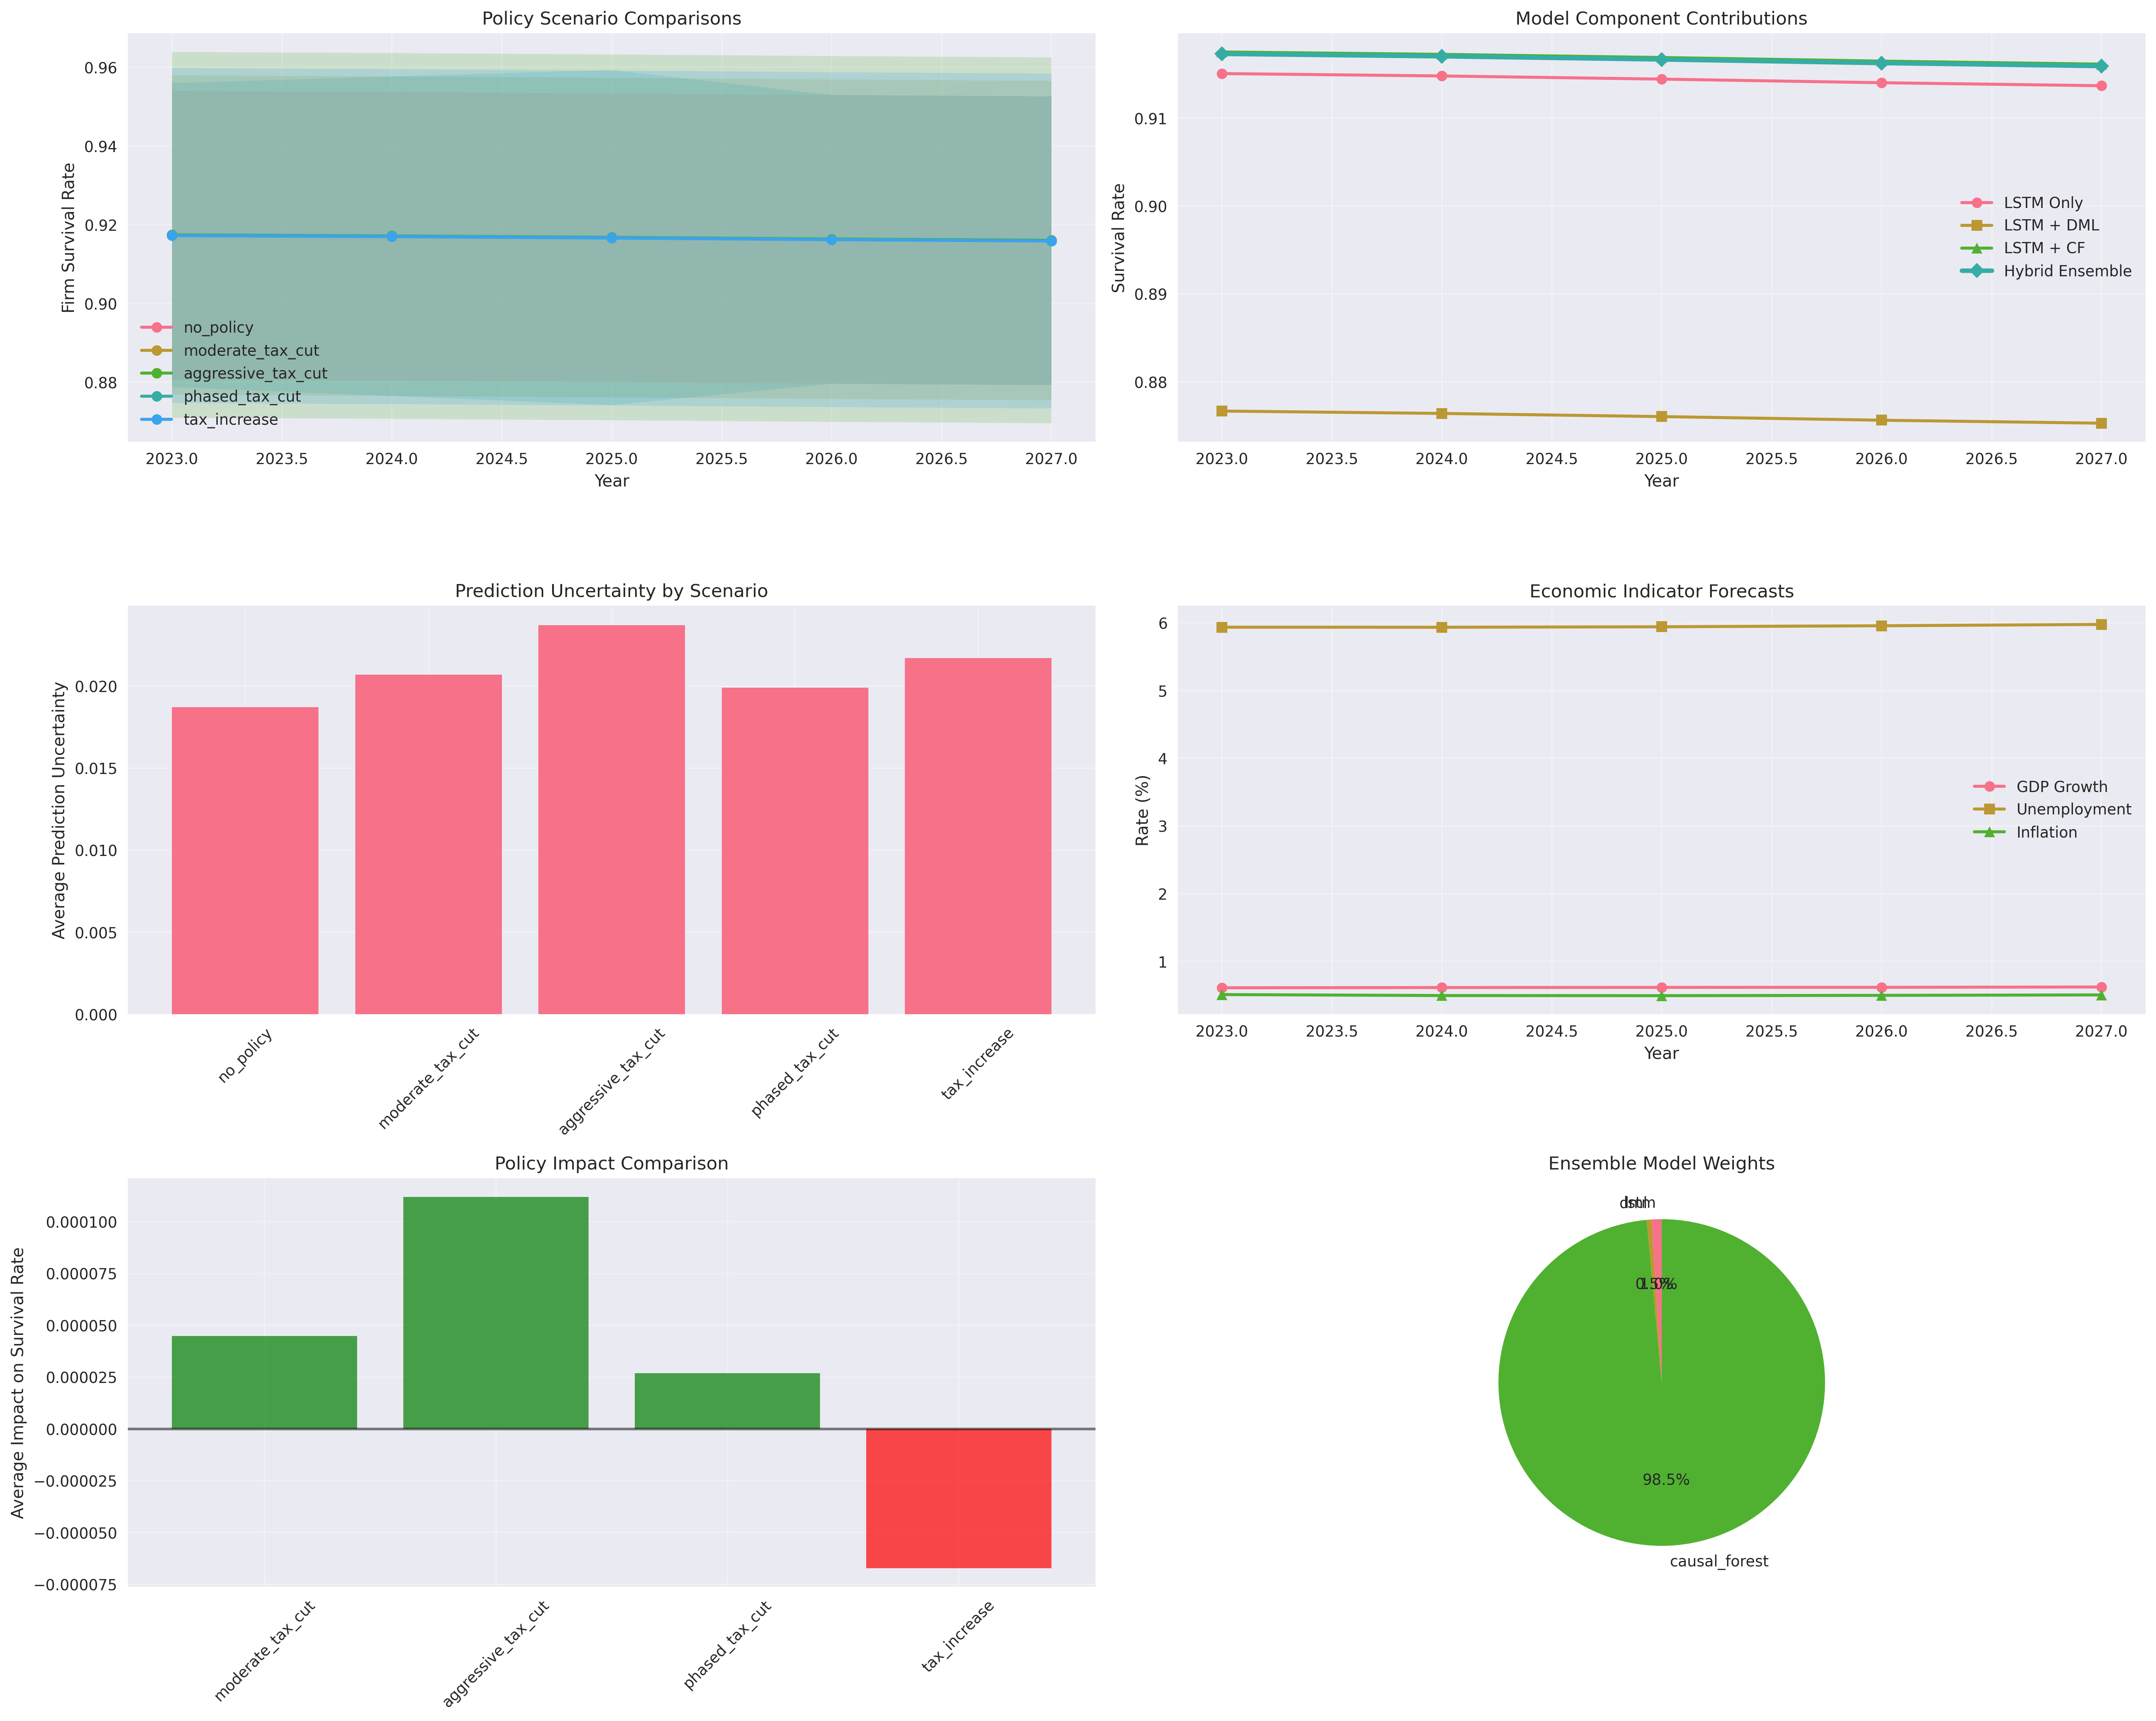
\includegraphics[width=\textwidth]{figures/hybrid_policy_analysis_comprehensive.png}
    \caption{Comprehensive Hybrid Policy Analysis Workflow}
    \label{fig:hybrid_policy_analysis_comprehensive}
\end{figure}

\begin{figure}[htbp]
    \centering
    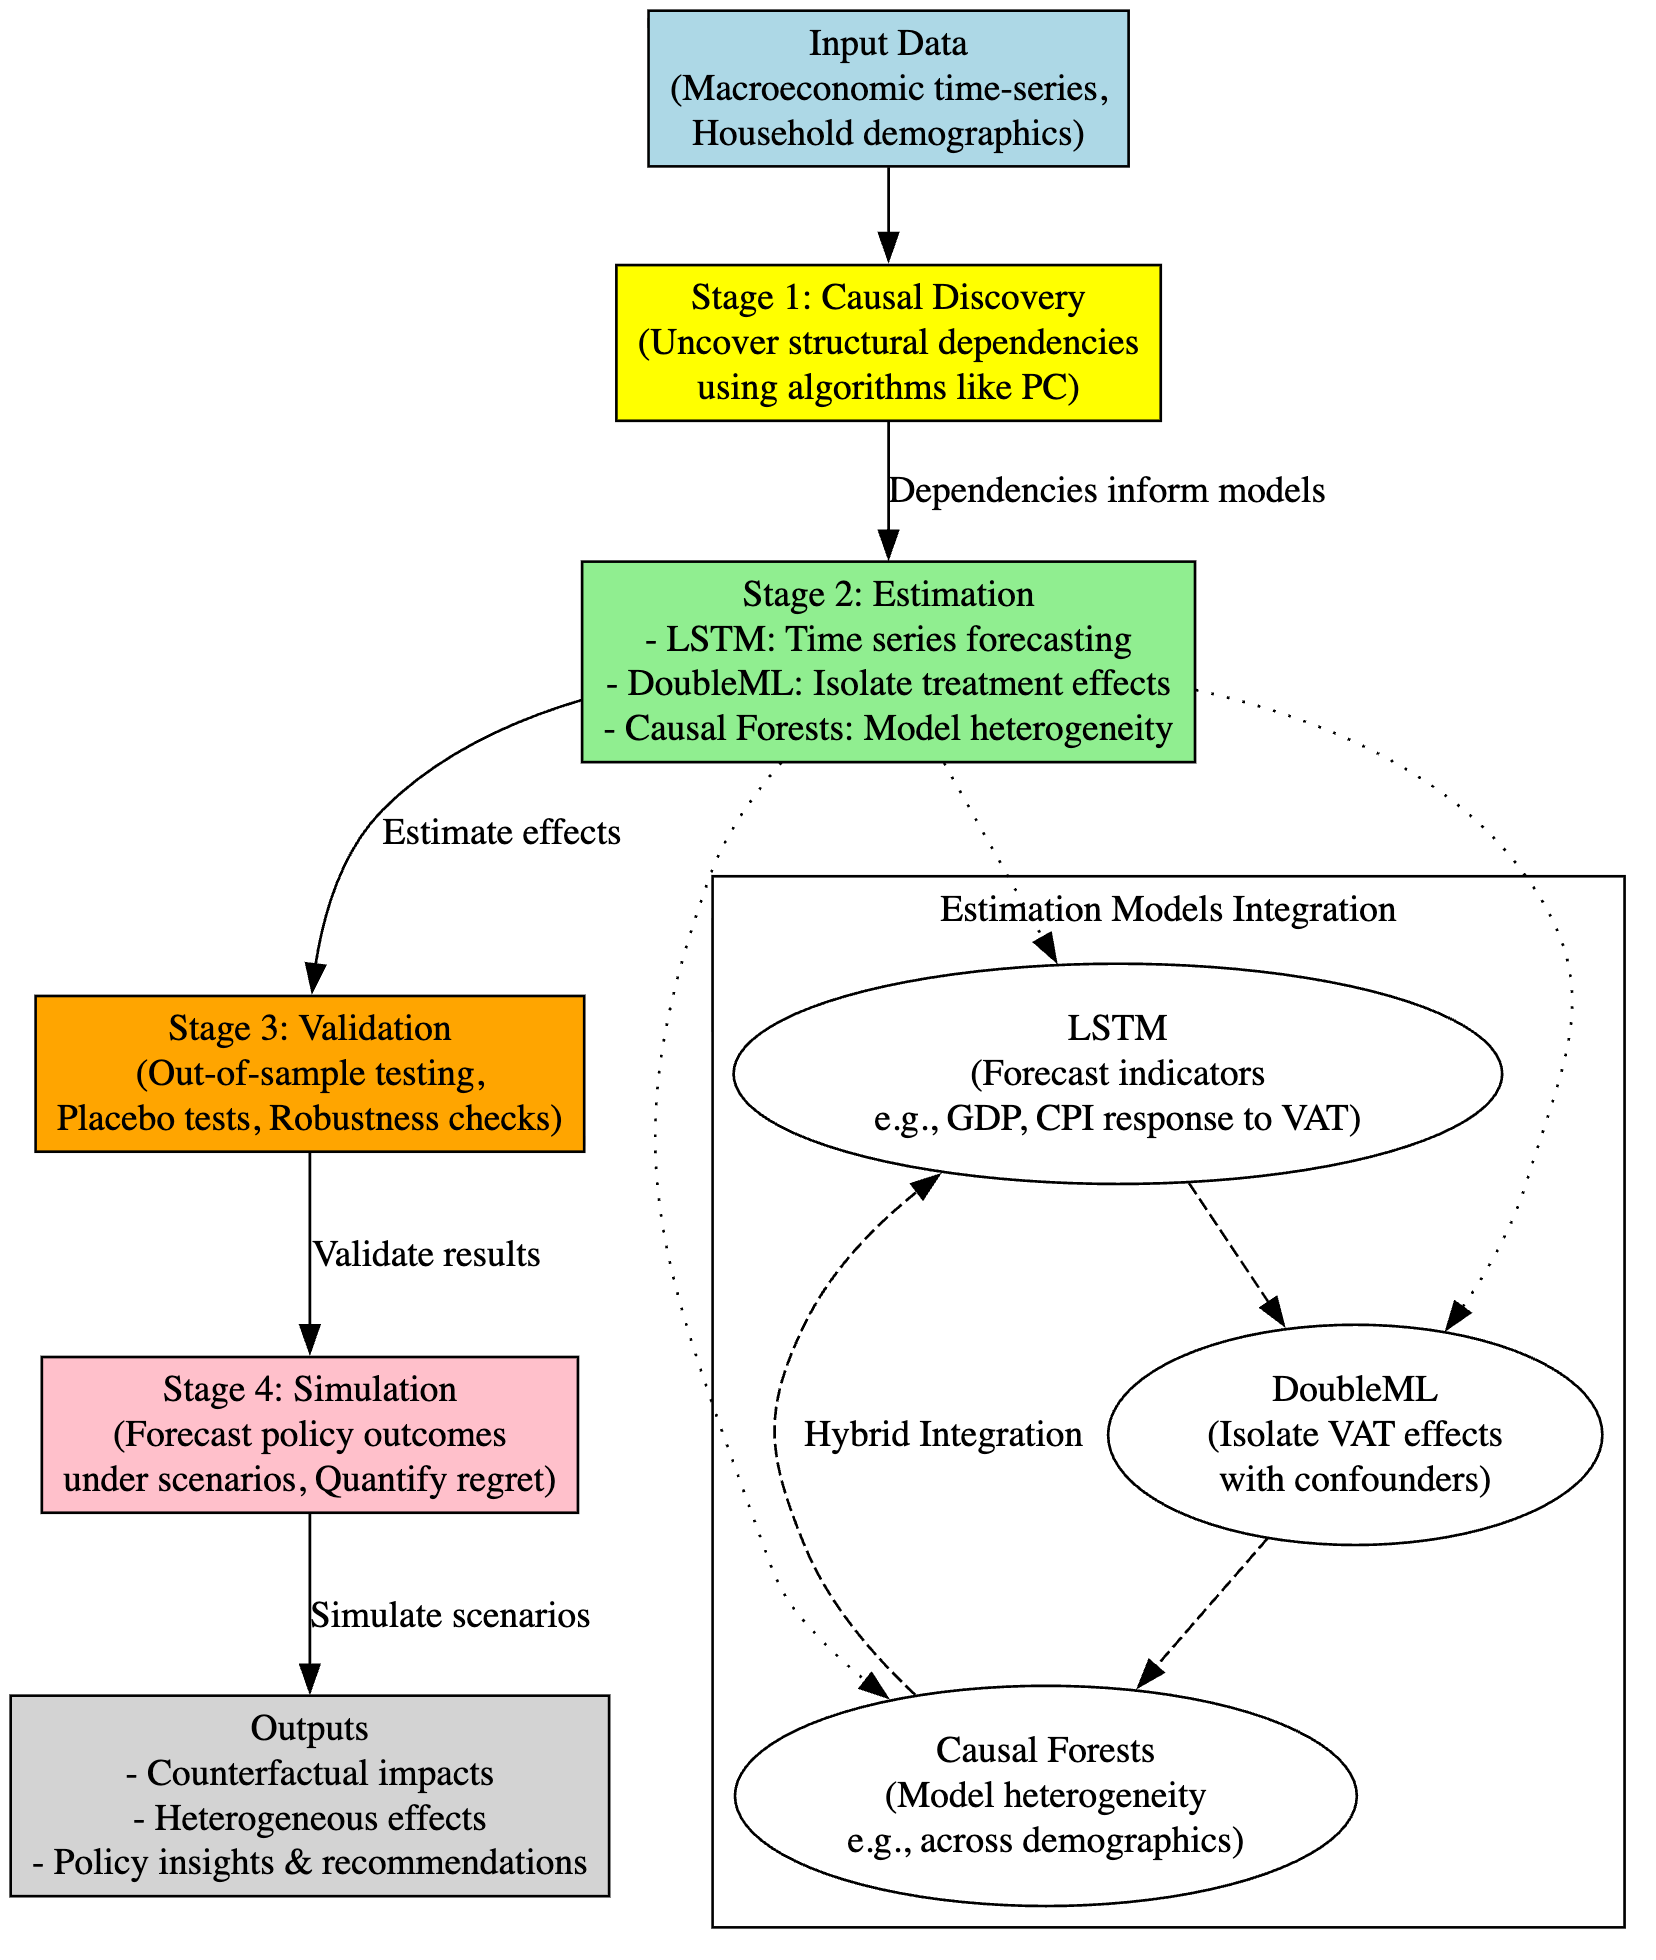
\includegraphics[width=\textwidth]{/Users/rishad/Downloads/ThesisPaperFinal/Defence-paper/thesis/images/wholestructure.png}
    \caption{Complete Hybrid Causal Machine Learning Model Architecture}
    \label{fig:complete_methodology}
\end{figure}

This comprehensive architecture demonstrates how causal discovery, DoubleML estimation, LSTM forecasting, and Causal Forest heterogeneity analysis work together to provide robust policy evaluation capabilities under uncertainty.

